\documentclass[unnumsec,webpdf,contemporary,large]{oup-authoring-template}
\usepackage{graphicx}
\usepackage{booktabs}
\usepackage{amsmath,amssymb}
\usepackage{url}
\usepackage{microtype}
\graphicspath{{../figures/}}
\DeclareUnicodeCharacter{03A8}{\ensuremath{\Psi}}
\newcommand{\TriFusionRM}{TriFusionRM}
\newcommand{\societylogo}{}
\journaltitle{Briefings in Bioinformatics}
\DOI{To be assigned}
\copyrightyear{2026}
\pubyear{2026}
\vol{XX}
\issue{x}
\access{Date to be assigned}
\appnotes{Original Paper}
\firstpage{1}
\title[TriFusionRM]{TriFusionRM: Integrating Sequence, Predicted RNA Structure, and RNA-Binding Protein Context for RNA Modification-Type Classification}
\author[1]{Author Name}
\address[1]{Department, Organization, City, Country}
\corresp{Corresponding author. email@example.com}
\abstract{RNA modifications regulate diverse aspects of RNA function, but modification types that share a central nucleotide can be difficult to distinguish from sequence alone. We developed TriFusionRM, a deep learning framework that integrates 41-, 101- and 201-nt sequence windows, predicted RNA structure and positional evidence from 30 RNA-binding proteins (RBPs) through three branches and gated residual fusion. On an RMBase-derived dataset of 1,082,044 sites, TriFusionRM achieved a test Macro AUPR of 0.9297 across eleven evaluable classes, exceeding the evaluated implementations of MultiRM (0.8694), TransRNAm (0.8421) and EvoRMD (0.8381). Its Macro AUPR was 0.01485 higher than that of the sequence-only model. On 96,352 external NaRMBench-derived sites spanning six classes, TriFusionRM achieved a Macro AUPR of 0.8085, an increase of 0.03877 over sequence only. Ablation and shuffled-input analyses supported the predictive value of site-matched RBP evidence, whereas predicted structure showed no consistent independent gain. Sequence perturbation further showed that test-replicated motifs influenced model predictions. These findings support the use of complementary biological context for RNA modification-type classification, with benefits that vary across modification classes.}
\keywords{RNA modification, multimodal learning, RNA secondary structure, RNA-binding proteins, sequence classification}
\begin{document}
\maketitle
\section{Introduction}

RNA modifications change the chemical properties of RNA and can influence splicing, stability, localization and translation \citep{ref1}. They occur in many RNA species and include m6A, m1A, m5C, pseudouridine ($\Psi$) and 2'-O-methylated nucleotides. Mapping these modifications helps us study how RNA is regulated. However, some modification types are rare, and different types can occur on the same base or share similar sequence patterns. These features make it difficult to distinguish modification types from sequence alone.

Experimental methods have provided maps of RNA modifications. MeRIP-seq \citep{ref2} identified regions enriched for m6A, and miCLIP \citep{ref3} improved the resolution of m6A and m6Am mapping. Other methods use chemical reactions to detect particular modifications, but they may be affected by incomplete reactions, sequence bias or uneven coverage \citep{ref4}. Nanopore sequencing can read native RNA and measure signals associated with modifications. For example, m6Anet \citep{ref5} detects m6A, CHEUI \citep{ref6} detects m6A and m5C, and TandemMod \citep{ref7} detects several modification types. These methods require suitable samples and sequencing coverage, and their accuracy depends on the modification and assay.

Computational prediction can help prioritize candidate modification sites. SRAMP \citep{ref8} uses sequence features and a random forest to predict m6A sites. iRNA-PseU \citep{ref9} uses local sequence information to predict $\Psi$ sites. WHISTLE \citep{ref10} combines sequence and genomic features for m6A prediction. These methods usually address one modification at a time. Deep-learning methods can learn sequence patterns to predict modification sites directly from data \citep{ref11}. PseUdeep \citep{ref12} applies deep learning to $\Psi$-site prediction. More recent methods include deepSRAMP \citep{ref13} for m6A prediction and Meta-PseU \citep{ref14} for $\Psi$ prediction from longer sequences. Their results depend on the labels and negative samples used for each task. Detecting one modification against unmodified sites is different from distinguishing among several modifications at annotated sites.

Other approaches predict more than one modification type. iMRM \citep{ref15} provides predictors for several modifications. MultiRM \citep{ref16} uses an attention-based multi-label model for twelve modifications. TransRNAm \citep{ref17} uses a Transformer-based multi-label model. MRM-BERT \citep{ref18} combines pretrained sequence representations with sequence features. EvoRMD \citep{ref19} uses RNA language-model representations and biological context for multiclass prediction. These studies broaden the range of predicted modifications. However, their tasks and input data differ, so their published scores cannot be compared directly.

It also remains unclear when information beyond sequence improves classification among annotated modification types. Longer sequence windows may help some classes but not others. Predicted RNA structure provides local pairing information, although it is derived from sequence \citep{ref20}. RBP binding profiles provide another source of context, including evidence from eCLIP experiments \citep{ref23}. 

Here, we present TriFusionRM to classify the modification type at sites already annotated as modified. The model combines centered 41-, 101- and 201-nt sequences, RNAfold-based structural features and positional eCLIP evidence from 30 RBPs. We evaluate sequence length, compare TriFusionRM with benchmark implementations and test the contribution of each evidence source. On the internal test set, TriFusionRM achieved a Macro AUPR of 0.9297, exceeding sequence-only prediction by 0.01485 and each evaluated benchmark implementation by at least 0.0603. We also examine motif-related prediction changes and transfer to an external dataset. The combined model improves average discrimination, although the benefit differs across classes. Evidence for site-matched RBP features is clearer than evidence for a consistent independent benefit from predicted structure.

\section{Materials and Methods}

\subsection{Datasets and preprocessing}

\subsubsection{Dataset 1. RMBase-derived modification-type benchmark}

We obtained human RNA modification sites from RMBase v3.0 \citep{ref24}. The twelve labels were Am, Cm, Gm, Um, m1A, m5C, m5U, m6A, m6Am, m7G, $\Psi$ and I. We removed duplicate sites within each modification type using genomic coordinate and strand. After checking the sequences and central bases, 1,087,461 sites had valid centered 41-nt sequences. For each class, the other modification classes form the one-versus-rest comparison group.

We clustered distinct 41-nt sequences with CD-HIT-est v4.8.1 \citep{ref25} at 80\% identity, using word length 5, global identity and at least 80\% coverage of both sequences (-c 0.8 -n 5 -G 1 -aS 0.8 -aL 0.8). The 1,065,639 distinct sequences formed 809,825 clusters. We assigned whole clusters to training, validation and test sets in an approximate 80:10:10 ratio. Next, we extracted centered 101-nt and 201-nt sequences from the GENCODE GRCh38 reference \citep{ref26}. For minus-strand sites, we used the reverse complement and checked that the central 41 nt matched the original sequence. We removed 5,417 sites that failed these checks. The final dataset contained 1,082,044 sites, including 865,582 for training, 108,251 for validation and 108,211 for testing. The longer sequences kept the split defined by the 41-nt clusters and were not clustered separately.

Each annotated site has one modification label. The final dataset contains 429 such coordinates. All 48 m6Am sites also have an Am annotation and belong to only two clusters. Of these, 47 are in training, one is in validation and none are in the test set. The model therefore has twelve outputs, but the internal test set supports evaluation of eleven classes. Only six m5U sites occur in the test set. Supplementary Table S1 shows the training, validation and test counts for each modification.

\subsubsection{Dataset 2. NaRMBench-derived external sites}

We obtained external sites from the real-sample NaRMBench dataset \citep{ref27}. The source files contained 371,244 annotated sites for m6A, I, $\Psi$, m5C, m1A and m7G. We standardized coordinates to GRCh38 after checking how each source indexed genomic positions. We removed duplicate sites, conflicting labels, sites overlapping Dataset 1 and sites with an incompatible central base, resulting in 186,055 sites. For each site, we extracted a centered 201-nt sequence and took its central 101-nt and 41-nt windows.

We then clustered the internal and candidate external 41-nt sequences together using MMseqs2 easy-linclust v13.45111 \citep{ref28} at 80\% identity and 80\% coverage. We removed 89,703 external sites from clusters that also contained an internal site, remaining 96,352 sites in 82,436 clusters. It included 54,597 m6A, 6,376 I, 20,212 $\Psi$, 5,765 m5C, 5,290 m1A and 4,112 m7G sites, which were used only for external evaluation. Their 41-, 101- and 201-nt sequences and corresponding structure and RBP features were supplied to the model in the same way as for Dataset 1. Supplementary Table S2 lists the filtering counts by class, and Supplementary Table S3 identifies the data sources and preprocessing steps. 

\subsection{Model building with three contextual evidence branches}

TriFusionRM has three parallel branches. The sequence branch processes three window lengths (Fig. 1A), the structural branch processes RNAfold features (Fig. 1B), and the RBP branch processes positional binding evidence (Fig. 1C). Each branch uses 128-dimensional representations. The sequence branch produces the main twelve-class prediction. The other two branches add gated residual contributions, as shown in Fig. 1D. In the sequence branch, the pooled CNN-BiGRU features are transformed to 128 dimensions using projection layers with GELU \citep{ref29} and layer normalization \citep{ref30}. The structural branch uses the same operations after pooling its graph features, while the RBP branch uses them when encoding positional input features. Fig. 1 summarizes these branches without depicting each operation as a separate box.

\begin{figure*}[!ht]\centering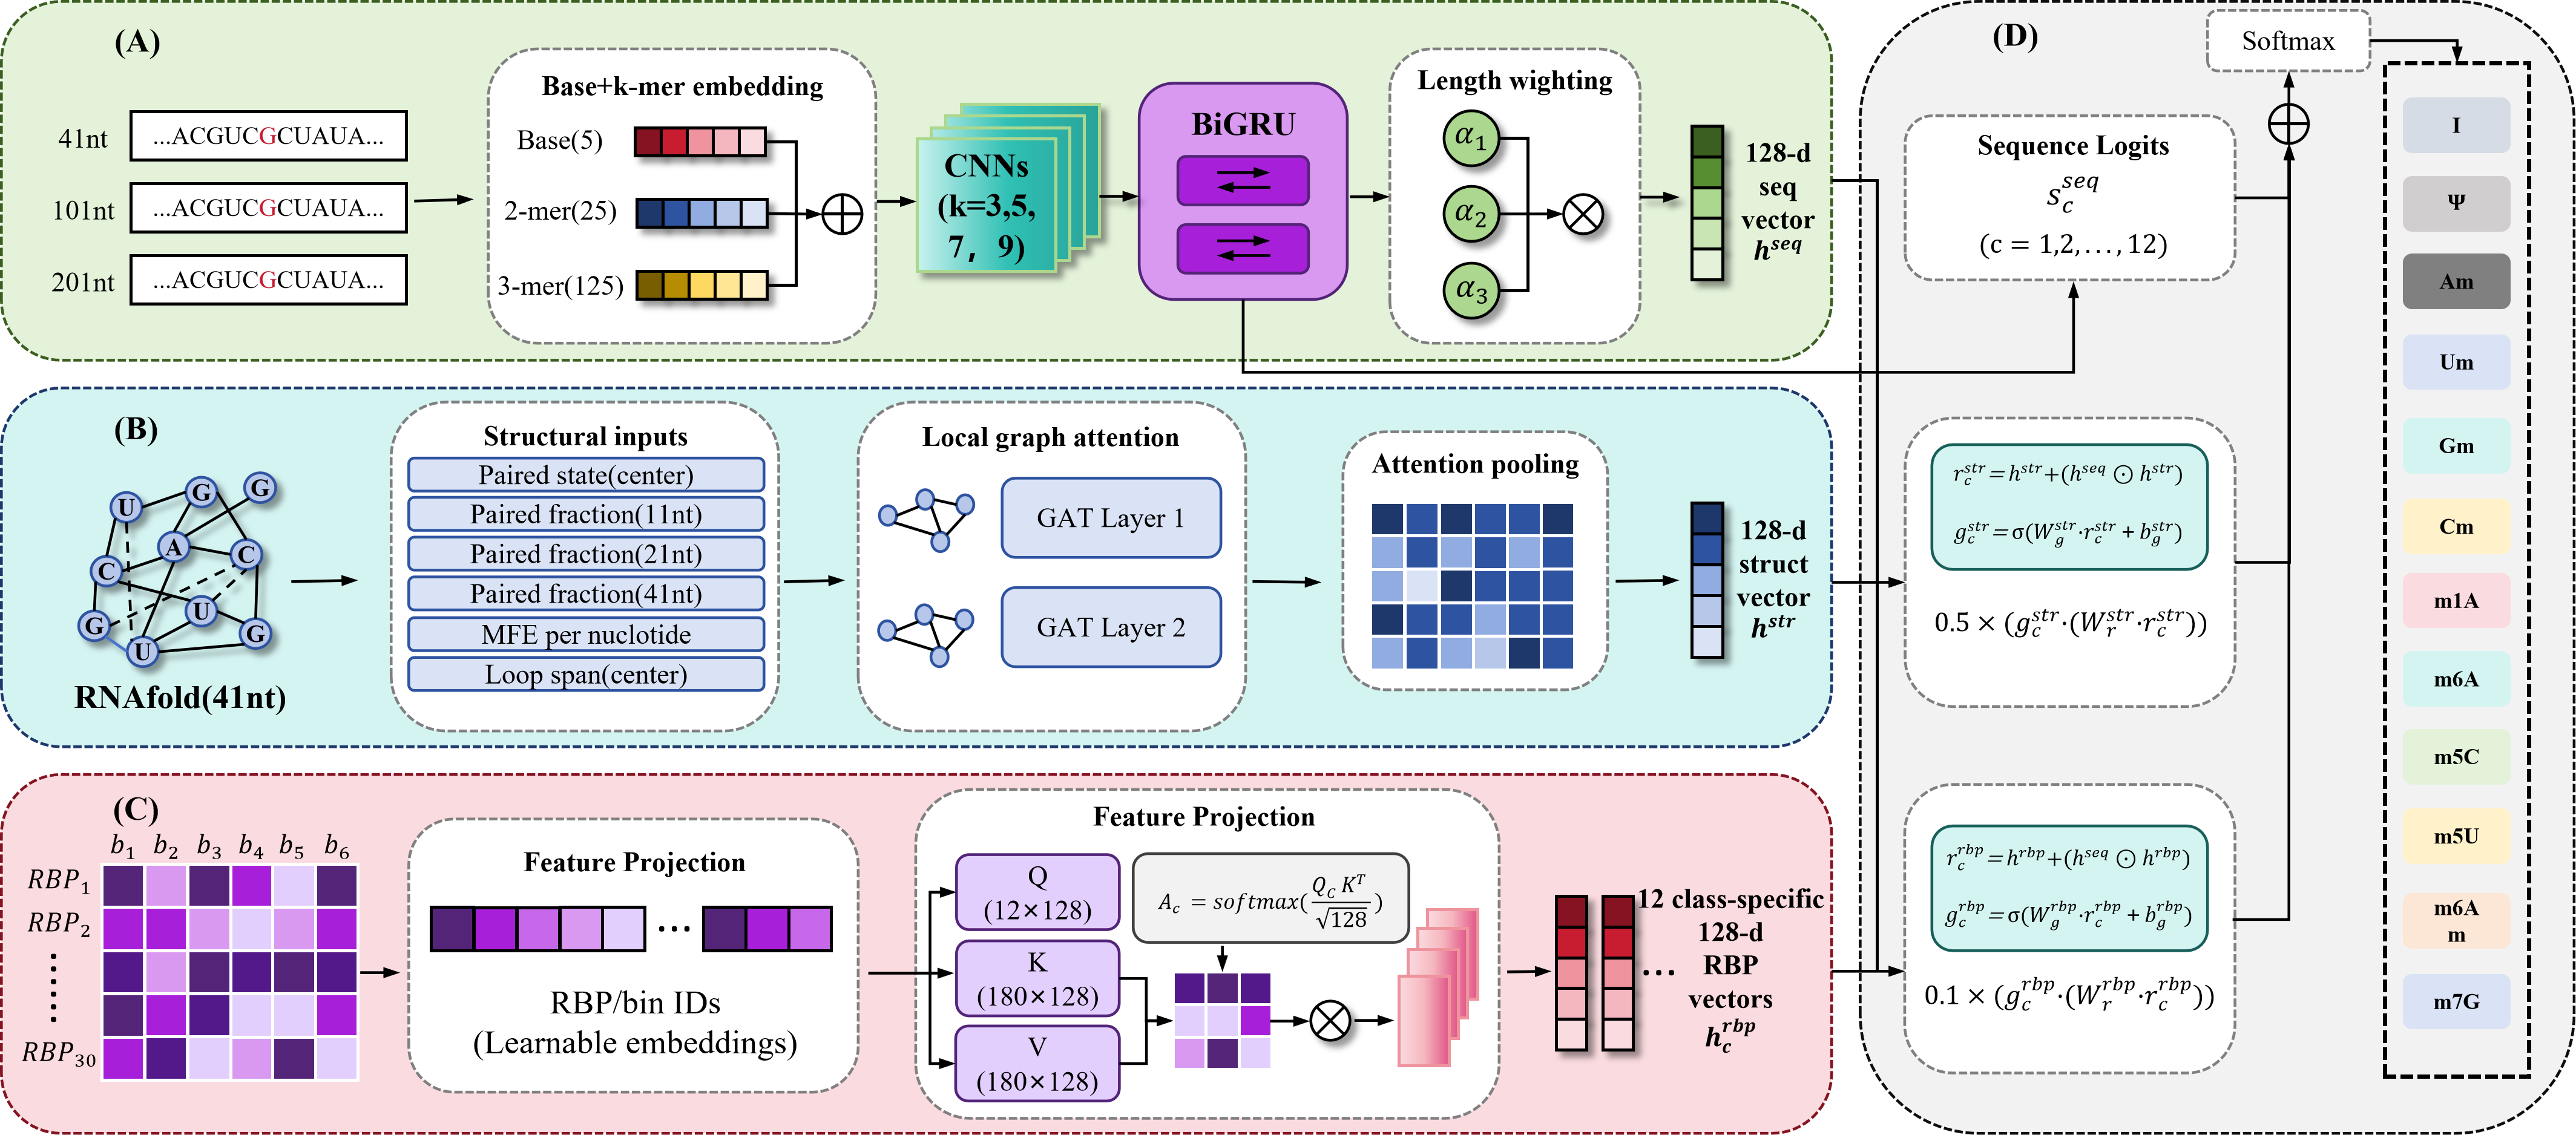
\includegraphics[width=0.82\textwidth]{../figures/figure1.png}\caption{Overview of the TriFusionRM architecture. TriFusionRM integrates three complementary sources of information for RNA modification-type classification. (A) The multi-scale sequence branch encodes centered 41-, 101- and 201-nt sequences using CNN--BiGRU networks and class-specific length weighting. (B) The structural branch extracts RNAfold-derived features through a local graph-attention network. (C) The RBP branch processes ENCODE eCLIP positional signals using class-conditioned attention. (D) Structural and RBP evidence are incorporated into sequence-based predictions through gated residual fusion, with scaling factors of 0.5 and 0.1, respectively. The fused logits are converted into probabilities over 12 RNA modification types using softmax.}\end{figure*}

\subsubsection{Multi-length sequence representation and encoding}

The sequence branch takes centered 41-, 101- and 201-nt windows. Nucleotides are encoded as A=1, C=2, G=3 and U/T=4, with 0 for unknown or padded positions. Overlapping 2-mer and 3-mer tokens start at each nucleotide and use base-5 encoding. Tokens past the right edge are padded with zeros. Separate trainable tables embed nucleotides, 2-mers and 3-mers into 128 dimensions. Their vectors are added at each position and then layer-normalized. A separate encoder processes each length, and learned weights combine the class logits.

Each length used its own encoder parameters. Four parallel one-dimensional convolutional neural network (CNN) branches, with kernel sizes 3, 5, 7 and 9 and 128 output channels each, used filters of different widths to capture short sequence motifs while preserving nucleotide positions. Their outputs were combined and mapped from 512 to 128 dimensions through a linear layer before the BiGRU. We summarized the BiGRU output vectors by concatenating the central-nucleotide vector, the mean vector over the central 11 nt, a center-conditioned attention pool and a global maximum pool. The attention pool scored each state jointly with the central-nucleotide vector through a tanh network followed by softmax. Two projection layers reduced the concatenated vector to the 128-dimensional representation.

A linear head converted each $z_L$ into twelve length-specific logits. A gating network received the concatenated vectors from all three lengths and produced a $12\times3$ array. Softmax over the three lengths produced weights $\alpha_{c,L}$.

\begin{equation}
s_c = \sum_{L\in W}\alpha_{c,L}s_{c,L},\qquad W=\{41,101,201\}.
\end{equation}

Here, $s_c$ is the sequence-branch logit for modification $c$, $s_{c,L}$ is its logit from window length $L$, and $\alpha_{c,L}$ is the learned weight assigned to that length. $W$ denotes the set of input lengths.

For interaction with the auxiliary branches, the gate weights were first averaged across classes. Their weighted average of $z_{41}$, $z_{101}$ and $z_{201}$ was then passed through a linear layer and normalized to form $z_{\mathrm{seq}}$.

\subsubsection{RNA structural representation and graph encoding}

The structural branch uses RNAfold \citep{ref22} to predict local folding from the centered 41-nt sequence. Each nucleotide is represented by a binary pairing status. We also calculate six features: the pairing status of the center, the fraction of paired nucleotides in the central 11 nt, 21 nt and full 41 nt, minimum free energy per nucleotide, and the span of unpaired nucleotides around the center. As shown in Fig. 1B, the pairing indicators and six summary features are passed to the structural encoder. The six features are standardized using statistics from the training set, which are also applied to the validation and test sets. The branch does not use nucleotide identity or learned position embeddings. These features summarize predicted local folding and the span of consecutive unpaired nucleotides around the center.

A linear layer maps binary pairing indicators to 128-dimensional nucleotide embeddings. Two graph-attention layers aggregate information from each nucleotide and its immediate neighbors along the RNA backbone \citep{ref32}. Boundary neighbors are masked. The layers use learned edge-type embeddings, attention-weighted aggregation, residual connections, layer normalization and a feed-forward block.

The structural representation, $z_{\mathrm{struct}}$, is obtained by concatenating the central-nucleotide embedding, the mean over the central 21 nt, a center-conditioned attention pool and the projected scalar descriptors, followed by a projection to 128 dimensions. Sequence--structure interaction was defined as

\begin{equation}
h_{\mathrm{int}} = [z_{\mathrm{seq}},\ z_{\mathrm{struct}},\ z_{\mathrm{seq}}\odot z_{\mathrm{struct}},\ |z_{\mathrm{seq}}-z_{\mathrm{struct}}|].
\end{equation}

Here, $h_{\mathrm{int}}$ is the sequence--structure interaction vector, $z_{\mathrm{seq}}$ is the pooled sequence representation, and $z_{\mathrm{struct}}$ is the structural representation. The symbol $\odot$ denotes element-wise multiplication, while the absolute-difference term gives the element-wise magnitude of the difference between the two representations.

A network with layers of 512, 256 and 12 dimensions transformed $h_{\mathrm{int}}$ to produce a structural residual $\delta_{\mathrm{struct}}$. The structural gate was computed separately from the concatenation of $z_{\mathrm{seq}}$ and $z_{\mathrm{struct}}$ using a 256-to-128-to-12 network with a sigmoid output. For class $c$, the structural contribution is

\begin{equation}
s^{\mathrm{seq+struct}}_c = s_c + 0.5\,g^{\mathrm{struct}}_c\delta^{\mathrm{struct}}_c.
\end{equation}

Here, $s^{\mathrm{seq+struct}}_c$ is the class-$c$ logit after sequence and structure fusion, $s_c$ is the sequence-only logit, $g^{\mathrm{struct}}_c$ is the structural gate, and $\delta^{\mathrm{struct}}_c$ is the class-specific structural residual. The factor 0.5 is the fixed structural scaling factor. A further linear layer mapped $h_{\mathrm{int}}$ to the joint context $h_{\mathrm{main}}$ used by the RBP fusion component.

\subsubsection{RBP positional representation and attention encoding}

We used ENCODE eCLIP \citep{ref23} data to describe RBP binding around each candidate site. For 30 RBPs, we divided the surrounding genomic region into six signed genomic-distance intervals, which are [-200, -100), [-100, -50), [-50, 0), [0, 50), [50, 100) and [100, 200) bp. For each RBP and interval, we calculated seven features covering peak presence, peak count, maximum and mean signal, closeness to the nearest peak summit, the fraction of the interval covered by peaks, and the fraction of peaks on the same strand as the site. Peak signals were set to nonnegative values before transformation, and intervals without peaks received zeros. As shown in Fig. 1C, these features form a positional input for the RBP branch. Supplementary Table S4 lists the RBPs and defines the seven features in detail.

The resulting $30\times6\times7$ tensor was mapped from seven features to 128 dimensions using a linear layer, GELU, layer normalization and dropout. The resulting feature vector was added to learned RBP-identity and interval-identity embeddings, forming 180 tokens. Twelve learned class queries computed scaled dot-product attention scores over the token representations, and their weighted token averages yielded class-conditioned RBP vectors.

As shown in Fig. 1D, the structural and RBP branches add separate gated residual contributions to the sequence logits. Their scaling factors are 0.5 and 0.1, respectively. The RBP residual combined a direct class-specific linear mapping with an interaction mapping of $[h_{\mathrm{main}},h_{\mathrm{RBP}},h_{\mathrm{main}}\odot h_{\mathrm{RBP}}]$. A shared network processed $[h_{\mathrm{main}},h_{\mathrm{RBP}}]$ to give the sigmoid gate. The final class logit is

\begin{equation}
\ell_c = s^{\mathrm{seq+struct}}_c + 0.1\,g^{\mathrm{RBP}}_c\bigl(\delta^{\mathrm{RBP}}_c+\delta^{\mathrm{interaction}}_c\bigr).
\end{equation}

Here, $\ell_c$ is the final logit for modification $c$, $s^{\mathrm{seq+struct}}_c$ is the sequence-plus-structure logit, $g^{\mathrm{RBP}}_c$ controls the RBP contribution, $\delta^{\mathrm{RBP}}_c$ is the direct RBP residual, and $\delta^{\mathrm{interaction}}_c$ is the residual from interactions between RBP features and the joint context. The RBP contribution is scaled by 0.1.

Softmax over all twelve logits produced class probabilities. This residual design allows the magnitude of auxiliary evidence to vary across sites and classes while retaining the sequence prediction as the common reference. Attention and gate values describe internal model weighting and are not treated as estimates of biological causality.

\subsection{Training strategy}

Models were trained on the frozen training partition with class-weighted cross-entropy. For each class c, we calculated a preliminary weight from the number of training sites:

\begin{equation}
w_c = \sqrt{\frac{N}{\max(n_c,1)}}.
\end{equation}

Here, $w_c$ is the preliminary weight for class $c$, $N$ is the total number of training sites, and $n_c$ is the number of training sites in class $c$. The max operation prevents division by zero. The weights were divided by their mean across the twelve classes.

\begin{equation}
\mathcal{L}_{\mathrm{total}}=\mathcal{L}_{\mathrm{main}}+0.1\mathcal{L}_{\mathrm{seq}}+0.05\mathcal{L}_{\mathrm{struct}}+0.05\mathcal{L}_{\mathrm{length}}+0.001R_{\mathrm{gate}}.
\end{equation}

Here, $\mathcal{L}_{\mathrm{total}}$ is the complete training objective. $\mathcal{L}_{\mathrm{main}}$, $\mathcal{L}_{\mathrm{seq}}$, $\mathcal{L}_{\mathrm{struct}}$ and $\mathcal{L}_{\mathrm{length}}$ are the main, sequence, structure and length-head losses, respectively. $R_{\mathrm{gate}}$ is the mean structural gate penalty. The numerical coefficients set the contribution of each auxiliary loss and penalty.

The main, sequence and structure losses use class-weighted cross-entropy. The length term is the mean cross-entropy across the three individual sequence heads, and $R_{\mathrm{gate}}$ is the mean structural sigmoid-gate value. Auxiliary losses for inactive branches were omitted. We optimized with AdamW at an initial learning rate of $3\times10^{-4}$ and weight decay $10^{-4}$. A cosine learning-rate schedule was applied for up to 50 epochs, dropout was 0.4, and gradient norms were clipped to 1. The batch size was 256 with four gradient-accumulation steps. Training stopped after eight epochs without a validation Macro AUPR improvement of at least $10^{-4}$, and the validation-selected checkpoint was used for testing. Seed 42 defines the primary comparisons. Seeds 17 and 73 quantify training variability where available. Macro AUPR was the primary evaluation metric. We also report Macro AUC, per-class precision, recall, F1, MCC, support, balanced accuracy and global MCC. The metric formulas and the distinction between per-class mean MCC and global MCC are shown in the Supplementary Information. Paired cluster resampling and multiple-comparison correction are described in the Supplementary Information. Final-model training settings are listed in Supplementary Table S5.

\section{Results}

\subsection{Sequence-window length and multi-length integration}

We first tested whether sequence-window length changed classification performance without structure or RBP inputs. Three sequence-only models used 41-, 101- or 201-nt windows. They shared the same encoder design, class weighting, validation-based checkpoint selection and training, validation and test sites. All sites retained the split defined by 41-nt clusters. Single-window models used a batch size of 1,024. The multi-length model used three separate encoders with a combined effective batch size of 1,024. As shown in Table 1 and Fig. 2A, the 101-nt sequence-only model achieved the highest Macro AUPR of 0.9151. This was 0.0112 higher than the 41-nt model and 0.0186 higher than the 201-nt model. The three-length model reached 0.9149, which was close to the 101-nt result. Fig. 2B shows that the best length differed among classes. For example, the 201-nt model had the highest Cm AUPR, whereas three-length fusion had the highest Am AUPR. The 101-nt advantage was therefore an average result, not a uniform gain across modifications. Per-class scores for the 41-, 101- and 201-nt models and the three-length model are provided in Supplementary Tables S6-S9, respectively. We kept the three-length sequence branch as the common baseline for testing structure and RBP inputs.

\begin{table*}[!ht]
\caption{Sequence-only performance across input lengths.}\centering
\fontsize{7.5}{9}\selectfont
\setlength{\tabcolsep}{3pt}
\setlength{\arrayrulewidth}{0.5pt}
\renewcommand{\arraystretch}{1.18}
\begin{tabular}{lrrrr}
\hline
Input length (nt) & Macro AUPR & Macro F1 & Global MCC & Balanced accuracy \\
\hline
41 & 0.9039 & 0.8484 & 0.9609 & 0.8737 \\
101 & 0.9151 & 0.8624 & 0.9617 & 0.8959 \\
201 & 0.8965 & 0.8632 & 0.9641 & 0.8839 \\
41 / 101 / 201 & 0.9149 & 0.8558 & 0.9629 & 0.8880 \\
\hline
\end{tabular}
\end{table*}

\begin{figure*}[!ht]\centering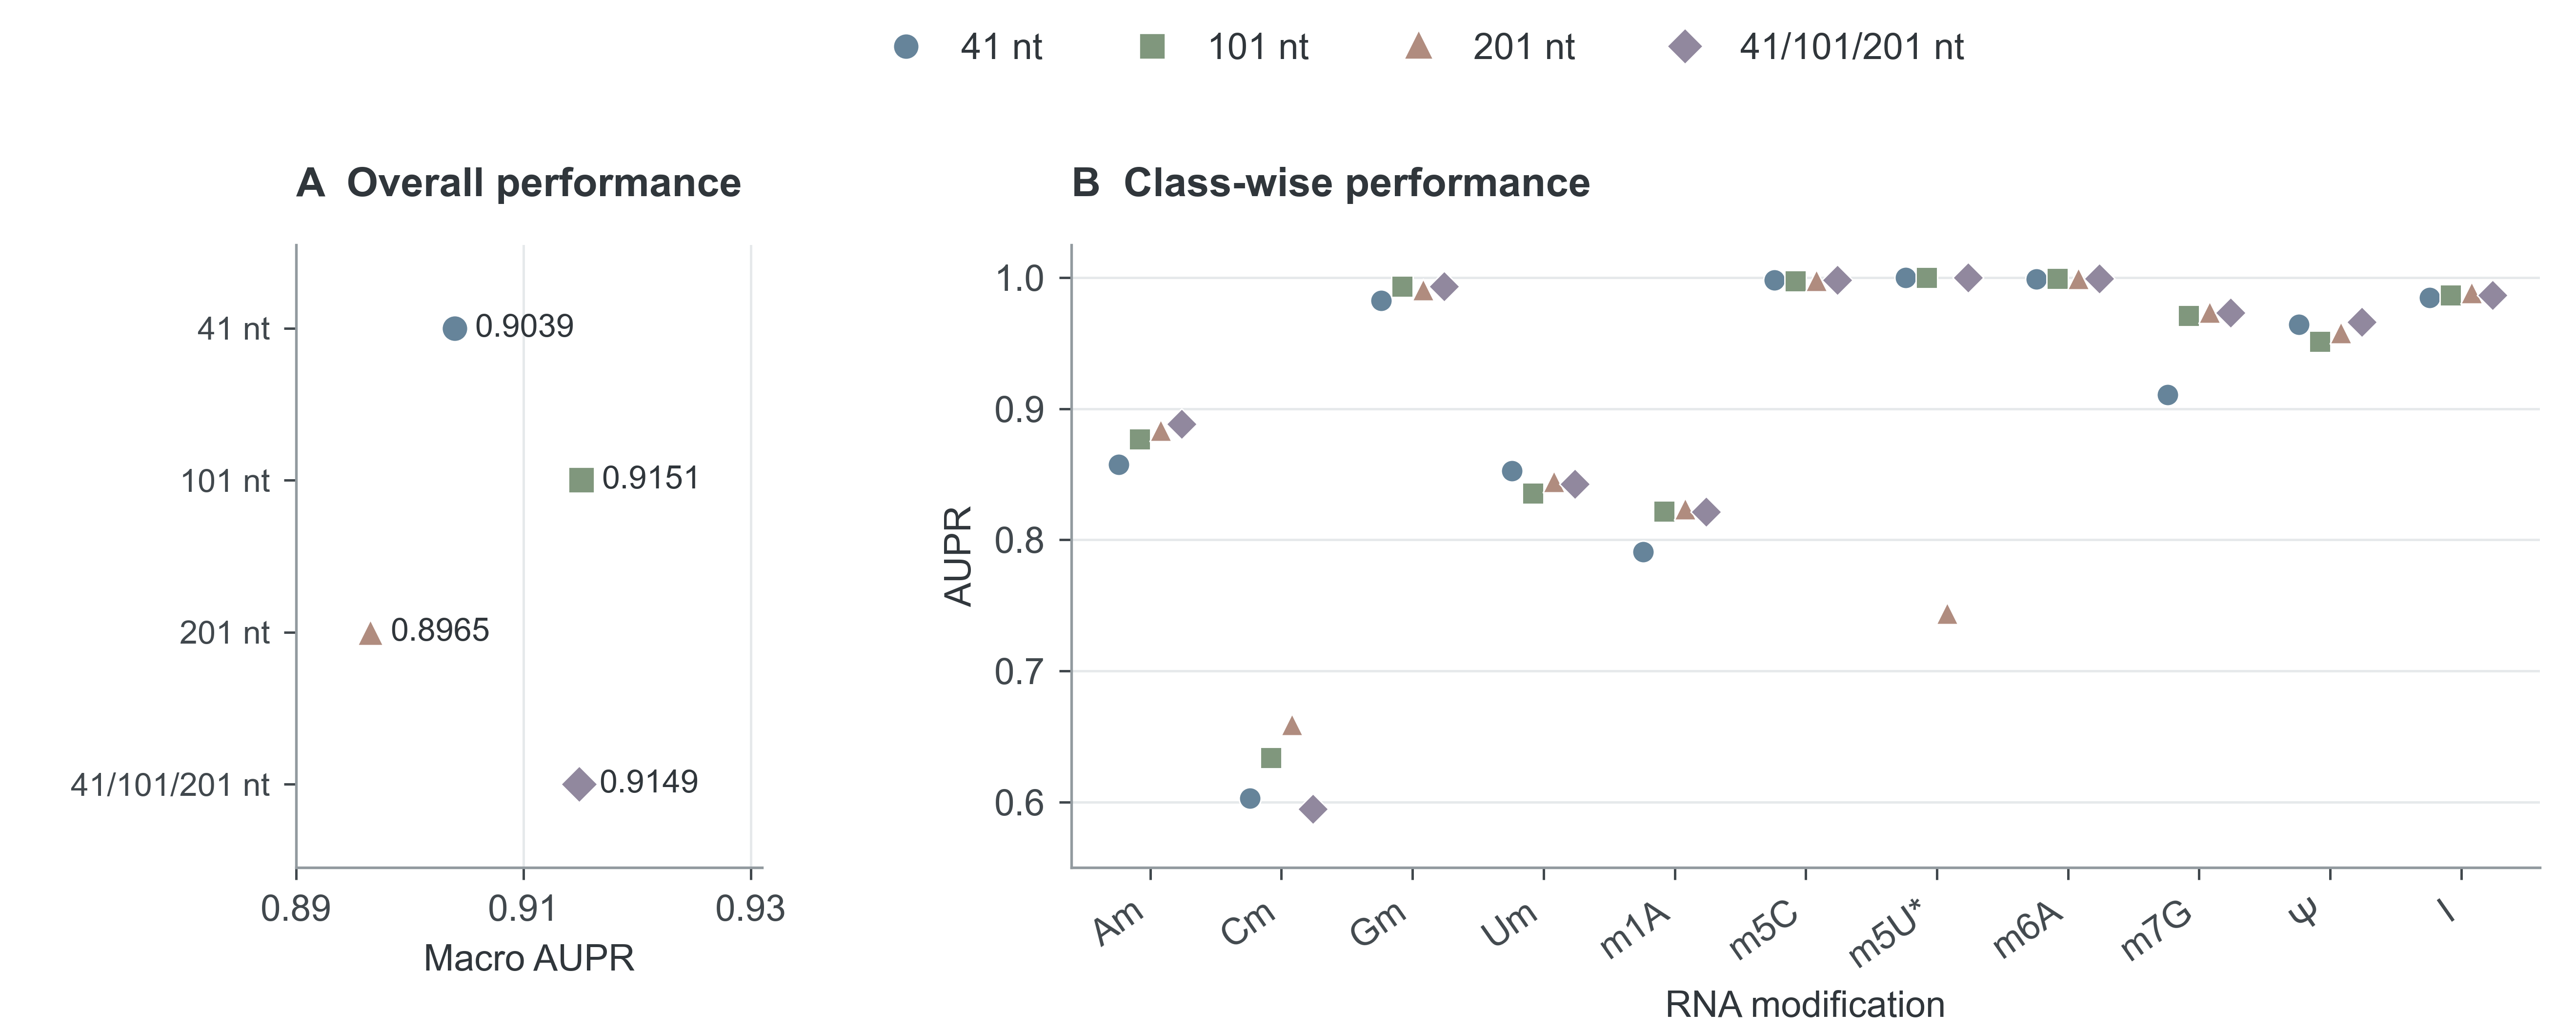
\includegraphics[width=0.82\textwidth]{../figures/figure2.png}\caption{Sequence-only prediction performance across input lengths. (A) Macro AUPR is the unweighted mean of class-wise AUPR over the 11 evaluable modification classes, with values corresponding to Table 1. (B) Class-wise AUPR is shown for 41-, 101- and 201-nt models and their multi-length integration. Colors and marker shapes identify the four input configurations. All points are seed 42 test estimates from validation-selected checkpoints evaluated on the same 108,211 sites. No across-seed uncertainty is implied. The displayed axes are restricted to the observed score ranges. All input lengths inherit the 41-nt cluster partition. m6Am is omitted because it has no test positives. The asterisk marks m5U, which has only six test sites.}\end{figure*}

\subsection{Comparison with established benchmark methods}

We compared TriFusionRM with three multi-modification benchmarks, MultiRM \citep{ref16} using recurrent sequence modeling and attention, TransRNAm \citep{ref17} using a Transformer, and EvoRMD \citep{ref19} combining RNA language-model features with biological context. The MultiRM and TransRNAm implementations used their core architectures, supplied embeddings and 41-nt input. The EvoRMD implementation used a frozen RNA-FM encoder and limited context features. All four methods were evaluated on exactly the same 108,211 test sites and labels. MultiRM and TransRNAm predictions were restricted from their 108,738-site sets to this common set. The input adaptations and training settings for each implementation are detailed in Supplementary Table S10. 

The performance is shown in Table 2 and Fig. 3. TriFusionRM achieved a Macro AUPR of 0.9297, exceeding MultiRM by 0.0603, TransRNAm by 0.0877 and EvoRMD by 0.0917 on the test set. The improvements over all three benchmark implementations remained statistically significant in paired cluster-bootstrap comparisons. Per-class precision, recall, F1 and AUPR are reported for the four implementations in Supplementary Tables S11-S14, and the corresponding paired intervals and adjusted P values are given in Supplementary Table S15.

\begin{table*}[!ht]
\caption{Performance of TriFusionRM and benchmark implementations.}\centering
\fontsize{7.5}{9}\selectfont
\setlength{\tabcolsep}{3pt}
\setlength{\arrayrulewidth}{0.5pt}
\renewcommand{\arraystretch}{1.18}
\begin{tabular}{lrrrrrr}
\hline
Model & Macro AUPR & Macro AUC & Macro F1 & Macro precision & Macro recall & Macro MCC \\
\hline
TriFusionRM & 0.9297 & 0.9984 & 0.8646 & 0.8573 & 0.8827 & 0.8648 \\
MultiRM & 0.8694 & 0.9961 & 0.8331 & 0.8487 & 0.8308 & 0.8332 \\
TransRNAm & 0.8421 & 0.9970 & 0.7503 & 0.7203 & 0.8141 & 0.7543 \\
EvoRMD & 0.8381 & 0.9957 & 0.8032 & 0.8165 & 0.8011 & 0.8000 \\
\hline
\end{tabular}
\end{table*}

\begin{figure*}[!ht]\centering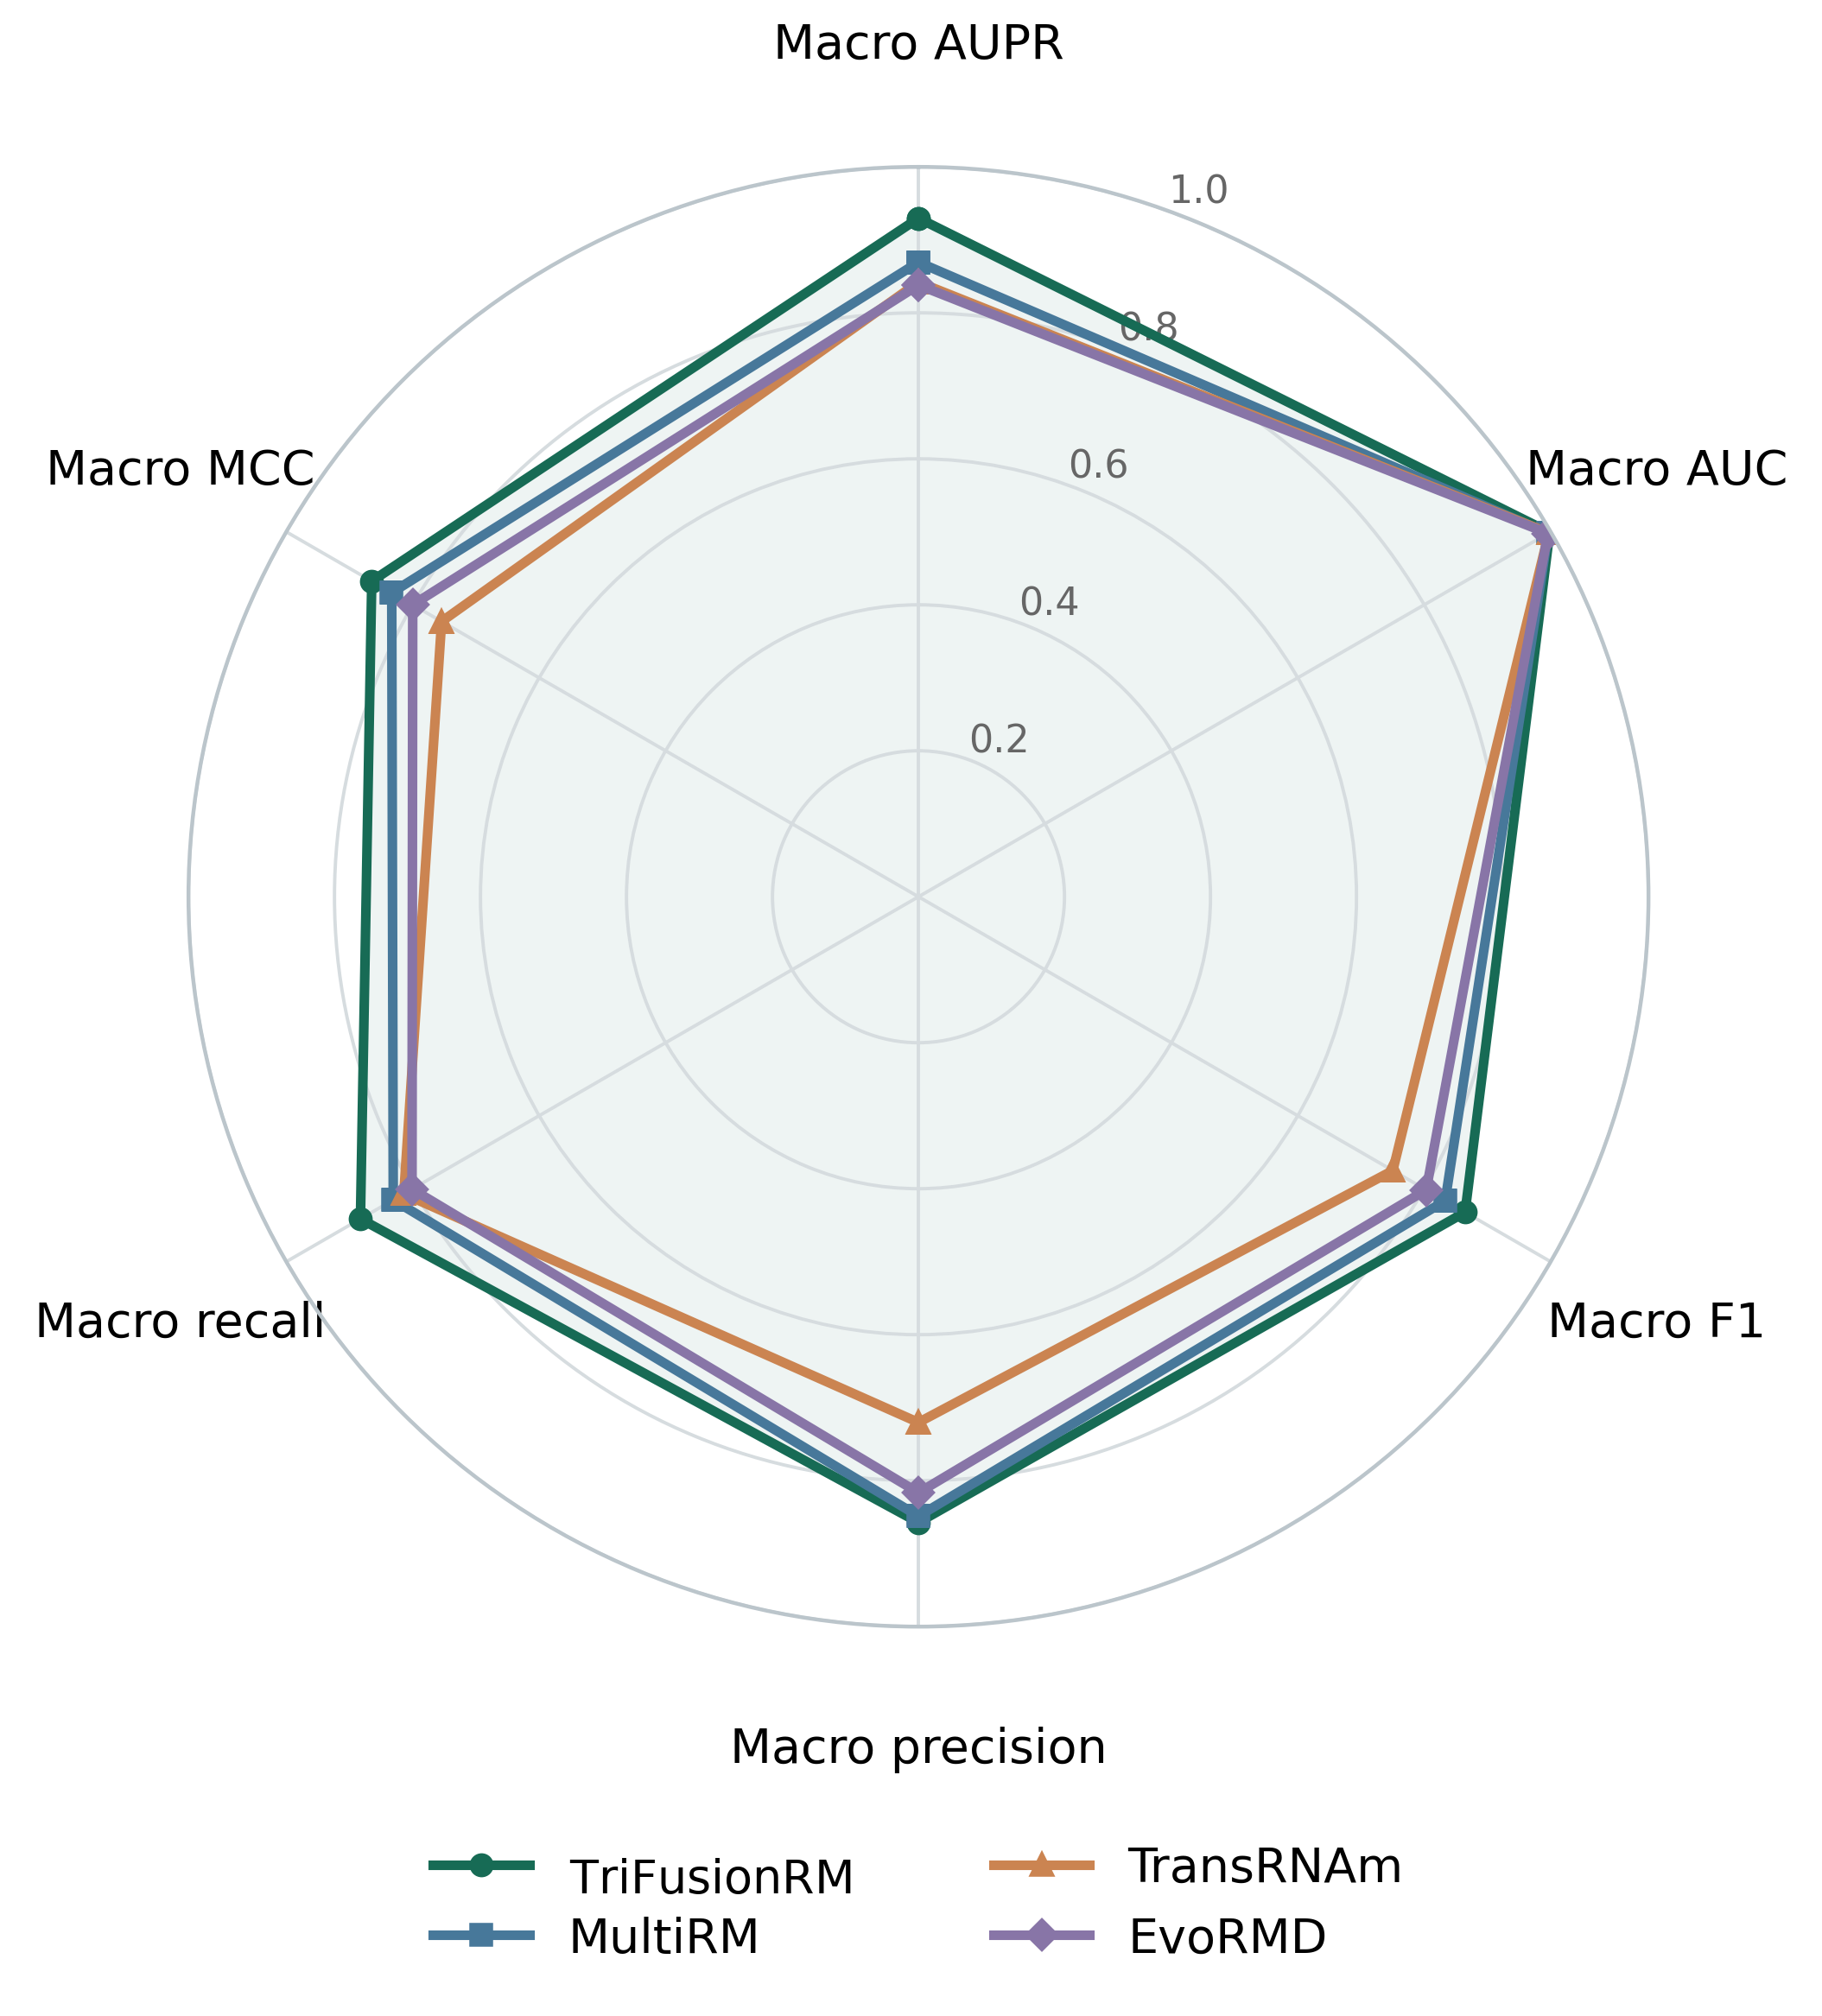
\includegraphics[width=0.50\textwidth]{../figures/figure3_TriFusionRM.png}\caption{Performance comparison of TriFusionRM and benchmark implementations. The radar plot shows Macro AUPR, Macro AUC, Macro F1, Macro precision, Macro recall and Macro MCC for TriFusionRM, MultiRM, TransRNAm and EvoRMD on the shared internal test set. Values farther from the center indicate higher scores.}\end{figure*}

\subsection{Contributions of structural and RBP evidence}

To assess the input sources, we compared sequence only, sequence plus structure, sequence plus RBP and the full TriFusionRM model. The result is shown in Table 3. The full model reached a Macro AUPR of 0.92972, a gain of 0.01485 over sequence only. Adding structure alone changed Macro AUPR by +0.00043, from 0.91487 to 0.91531. Adding RBP alone changed it by +0.00433, to 0.91921. In contrast, adding RBP when structure was already present increased Macro AUPR by +0.01442.

\begin{table*}[!ht]
\caption{Modality ablations with the multi-length sequence backbone.}\centering
\fontsize{7.5}{9}\selectfont
\setlength{\tabcolsep}{3pt}
\setlength{\arrayrulewidth}{0.5pt}
\renewcommand{\arraystretch}{1.18}
\begin{tabular}{lrrrr}
\hline
Input evidence & Macro AUPR & Macro F1 & Global MCC & Balanced accuracy \\
\hline
Sequence only & 0.9149 & 0.8558 & 0.9629 & 0.8880 \\
Sequence + structure & 0.9153 & 0.8538 & 0.9640 & 0.8743 \\
Sequence + RBP & 0.9192 & 0.8455 & 0.9628 & 0.9001 \\
TriFusionRM & 0.9297 & 0.8646 & 0.9684 & 0.8827 \\
\hline
\end{tabular}
\end{table*}

We next tested whether the auxiliary inputs needed to match each site. We trained control models after shuffling whole RBP tensors, structural inputs or the six RBP distance intervals. As shown in Fig. 4, authentic RBP evidence achieved a Macro AUPR of 0.92972, exceeding the shuffled-RBP control by 0.03110. The positive difference passed correction for Cm, Um, m1A, m6A and I. Site-matched RBP features contributed more strongly than the specific ordering of the six genomic-distance intervals. The effects of auxiliary inputs differed across modification types. Site-matched RBP evidence significantly improved AUPR for Cm, Um, m1A, m6A and I, whereas adding structure to sequence slightly improved I but reduced $\Psi$ AUPR. Paired estimates and adjusted P values are provided in Supplementary Tables S16--S19.

\begin{figure*}[!ht]
\centering
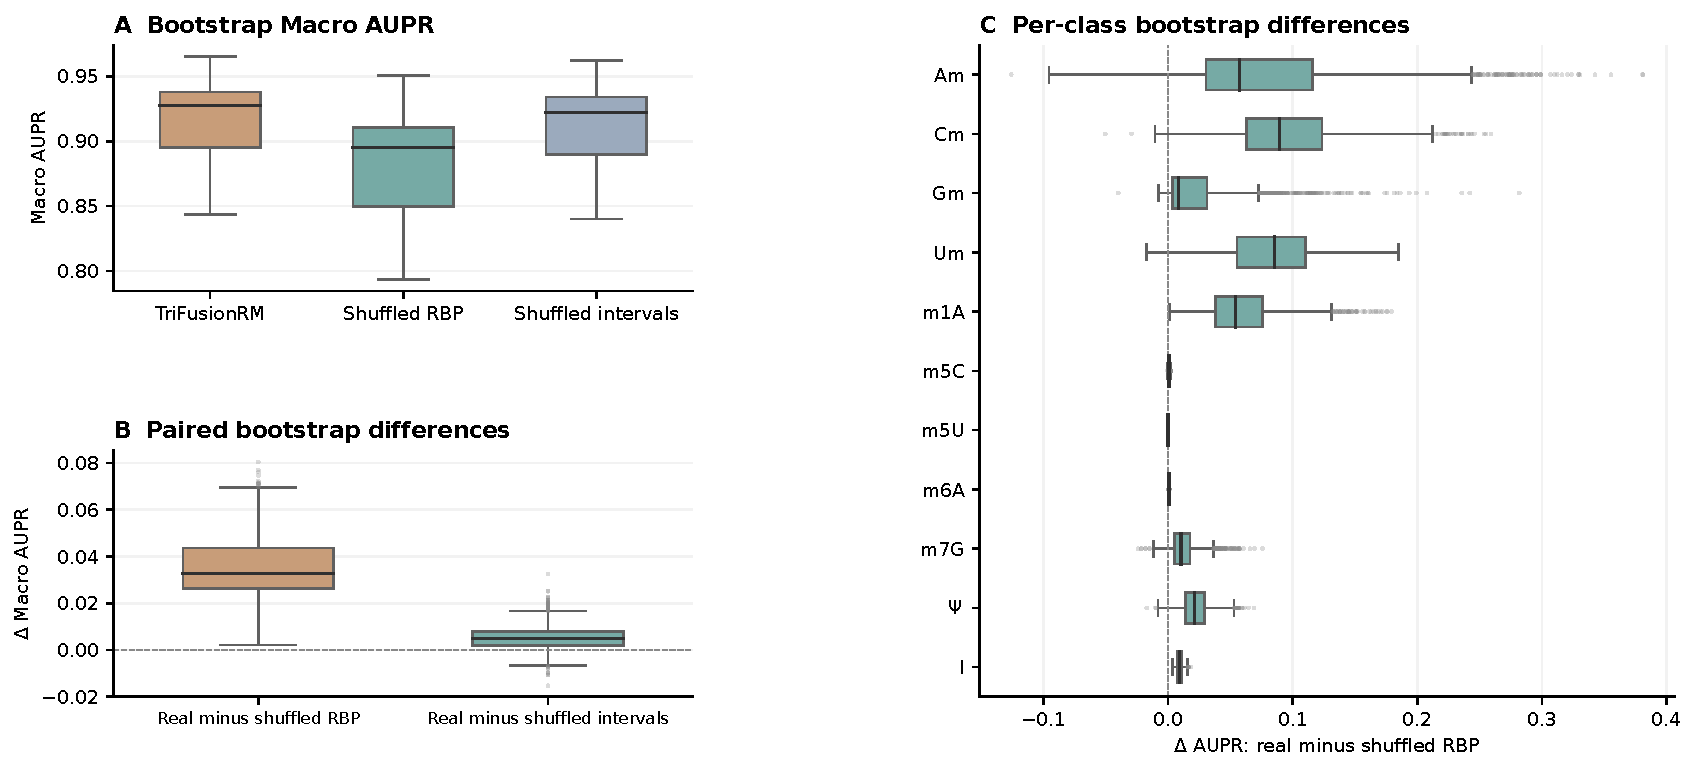
\includegraphics[width=\textwidth]{../figures/Figure4_boxplot.pdf}
\caption{RBP controls in no-pair TriFusionRM. A shows bootstrap Macro AUPR for the real-RBP model and trained shuffled-RBP and shuffled-distance-interval controls. B shows paired Macro AUPR differences, and C shows per-class real-minus-shuffled-RBP differences. Each box summarizes 2,000 matched cluster-bootstrap draws from the frozen test set, not independent training runs. Boxes span the 25th to 75th percentiles, lines mark medians, whiskers extend to the most extreme observations within 1.5 interquartile ranges, and dots show observations beyond the whiskers. Only draws retaining positive sites for all 11 evaluable classes were accepted. These boxplots are not 95\% confidence intervals; paired intervals and adjusted P values remain in Supplementary Tables S16 and S18. m6Am has no test positives.}
\end{figure*}

The structural results varied by class. Authentic structure exceeded shuffled structure by +0.00830 in Macro AUPR. The class-wise contrast was +0.00128 for I, while adding structure to sequence alone reduced $\Psi$ AUPR by 0.03395. Adding structure to sequence significantly improved I AUPR but reduced $\Psi$ AUPR. Neither the no-pair versus pair-edge comparison nor the gate-sharing comparisons showed a statistically supported difference in Macro AUPR. The pair-edge and gate-sharing comparisons in Tables S20--S22, and structural controls with uncertainty intervals in Supplementary Fig. S1.

\subsection{Internal and external predictive performance}

Having examined the contributions of different input sources, we further evaluated the predictive performance of TriFusionRM on internal and external datasets. The internal evaluation assessed overall classification performance, class-specific differences and variability across training seeds. The external evaluation examined whether the trained model could maintain its predictive advantage on data from a different source without retraining.

On the internal test set, TriFusionRM achieved Macro AUC 0.9984, Macro F1 0.8646 and balanced accuracy 0.8827. Most well-supported classes had high AUPR, but Cm reached 0.6694. The model reached 0.9997 for m6A, while the AUPR of 1.0000 for m5U rests on only six test sites. Across three training seeds, mean test Macro AUPR was 0.9276 with a sample standard deviation of 0.0037.

We applied the frozen TriFusionRM and sequence-only checkpoints to Dataset 2 without retraining or selecting a model on external labels. We generated structure and RBP features using the same definitions as for Dataset 1. We kept all twelve output probabilities and averaged AUPR over the six classes present externally. 

On Dataset 2, TriFusionRM achieved a Macro AUPR of 0.80847, an increase of 0.03877 over sequence only. The largest gains were observed for I and m1A, while AUPR decreased for m6A, $\Psi$ and m7G and remained 1.0000 for m5C at the reported precision. Thus, the average gain was concentrated in particular modifications. Table 4 gives the external point estimates by class. The external Macro AUPR improvement was statistically significant and was driven by gains for I and m1A, despite significant decreases for m6A, $\Psi$, m5C and m7G, as detailed in Supplementary Table S23.

\begin{table*}[!ht]
\caption{Frozen-model performance on the external NaRMBench-derived set.}\centering
\fontsize{7.5}{9}\selectfont
\setlength{\tabcolsep}{3pt}
\setlength{\arrayrulewidth}{0.5pt}
\renewcommand{\arraystretch}{1.18}
\begin{tabular}{lrrr}
\hline
Modification & Test sites & Sequence-only AUPR & TriFusionRM AUPR \\
\hline
m6A & 54,597 & 0.9790 & 0.9727 \\
I & 6,376 & 0.5494 & 0.7523 \\
$\Psi$ & 20,212 & 0.9999 & 0.9969 \\
m5C & 5,765 & 1.0000 & 1.0000 \\
m1A & 5,290 & 0.1021 & 0.1553 \\
m7G & 4,112 & 0.9878 & 0.9735 \\
Macro & 96,352 & 0.7697 & 0.8085 \\
\hline
\end{tabular}
\end{table*}

\subsection{Statistical validation and sequence-level interpretation}

We tested whether the overall gain persisted when comparisons focused on modifications with the same central base. In this analysis, the full model exceeded sequence only by +0.01536 in Macro AUPR. Requiring at least ten positive test clusters per class, which excluded m5U, gave a difference of +0.01634. These results indicate that the average gain is not driven only by different central bases or by the six m5U test sites. The bootstrap comparisons resampled clusters while keeping paired predictions together. 

We also tested whether the model responded to local sequence patterns. A cluster-level analysis selected thirty 4-6-nt motifs in training using classes with the same central base as background. All thirty were confirmed in validation, and twenty were reproduced in the held-out test set. The reproduced set included two motifs for Am and three each for Um, m1A, m5C, m6A, $\Psi$ and I. Cm, Gm and m7G motifs were not reproduced in test. m5U and m6Am lacked enough independent positive clusters for this analysis. This test-set replication was concentrated in seven modification classes, whereas the Cm, Gm and m7G candidates remained validation-only. All 30 training-selected motifs were confirmed in validation, and 20 were significantly replicated in the independent test set, with class-level counts and enrichment results detailed in Supplementary Tables S24--S26.

For each of the twenty reproduced motifs, we retained at most one site per motif, class and cluster. We compared ten motif-disrupting changes with ten matched random changes per site. We protected the central base, changed the same positions in all three sequence windows and kept structure and RBP inputs fixed. As shown in Fig. 5, motif disruption caused a larger decrease in the target-class logit than matched random changes for all twenty motifs after correction. We averaged repeated observations within clusters before analysis. The perturbation analysis measures model sensitivity to the test-replicated motifs. Motif disruption reduced target-class logits significantly more than matched random changes for all seven modifications and all 20 motifs, with the corresponding results reported in Supplementary Tables S27 and S28.

\begin{figure*}[!ht]
\centering
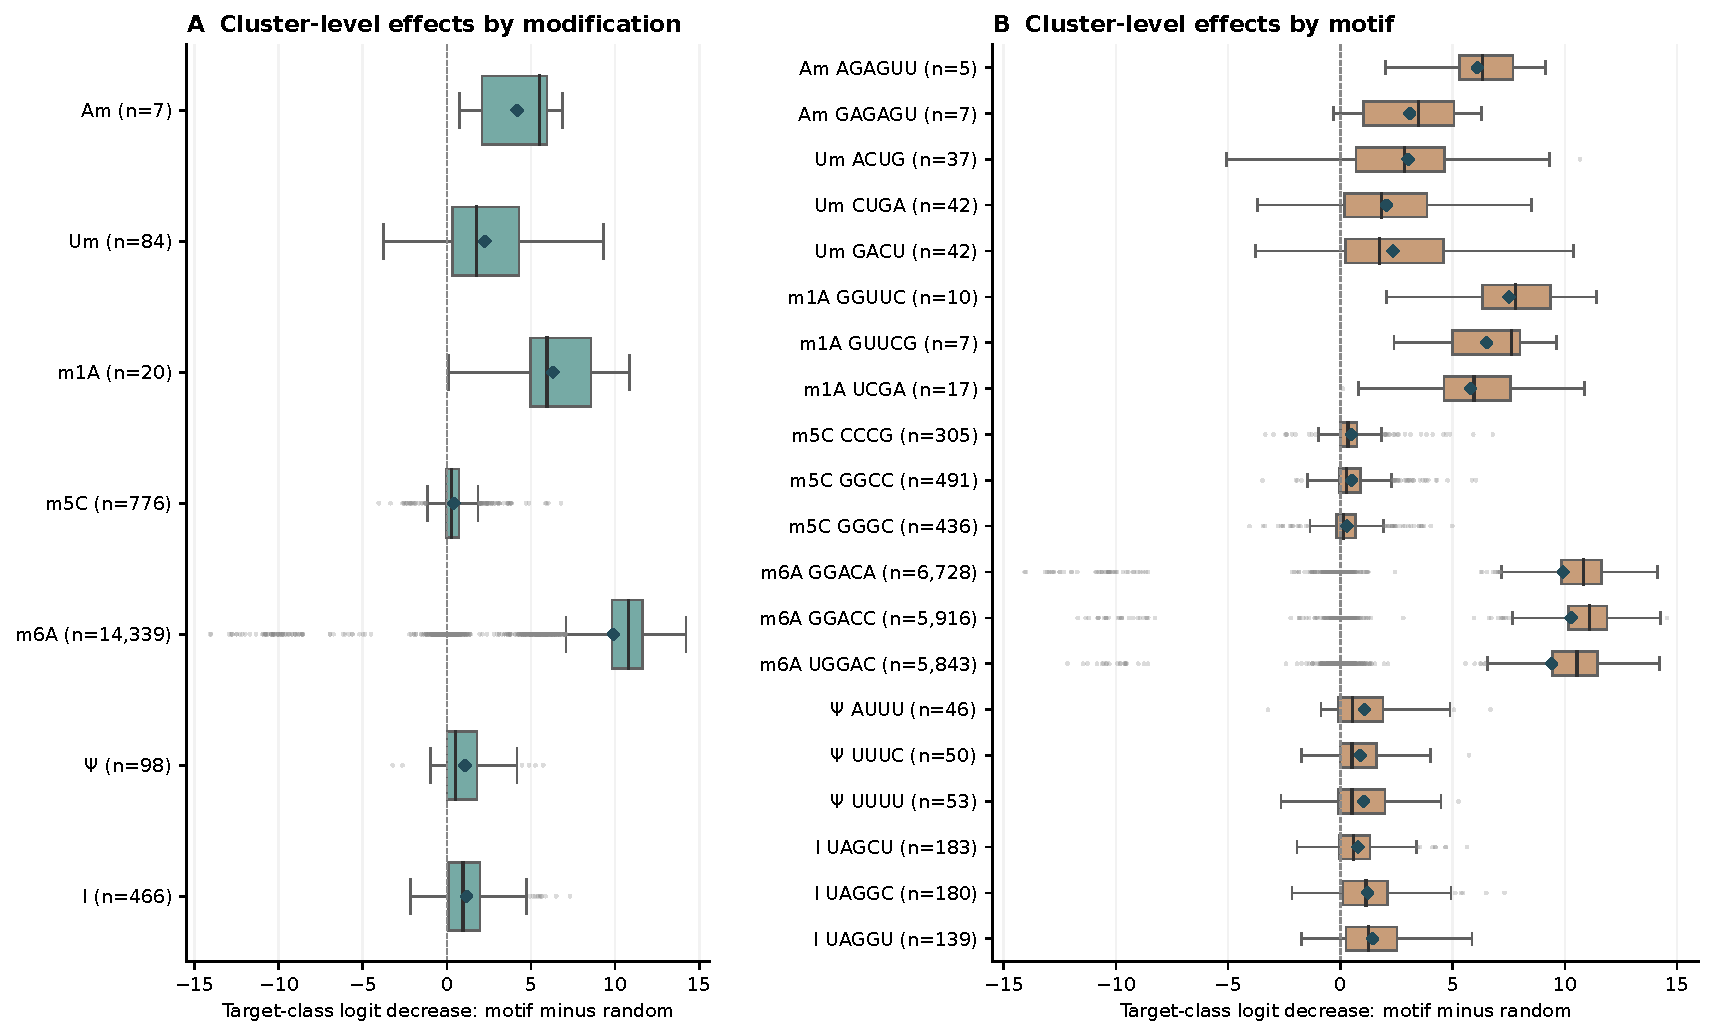
\includegraphics[width=\textwidth]{../figures/Figure5_boxplot.pdf}
\caption{Cluster-level sensitivity to motif disruption in no-pair TriFusionRM. A summarizes contrasts after averaging motif-site observations within each modification and cluster. B summarizes the fixed set of 20 test-replicated motifs after averaging within each motif and cluster. The contrast is the target-class logit decrease after motif disruption minus that after matched random disruption, with 10 perturbations averaged per condition and site. Each observation is a cluster-level contrast. Boxes span the 25th to 75th percentiles, center lines mark medians, whiskers extend to the most extreme observations within 1.5 interquartile ranges, and dots show observations beyond the whiskers. Diamonds mark means, and n denotes contributing clusters. These distributions show cluster-to-cluster variation rather than confidence intervals of the mean. The center base was protected, edits were synchronized across windows, and structure and RBP inputs were fixed. Confidence intervals and adjusted P values remain in Supplementary Tables S27 and S28. Am is supported by seven clusters overall.}
\end{figure*}

The frozen model was evaluated for $\Psi$ and other U modification discrimination against a retrained 32-model Meta-PseU ensemble. TriFusionRM reached an AUPR of 0.9624, a difference of +0.0117 from Meta-PseU. This task-specific comparison assesses discrimination among U-centered modifications. TriFusionRM achieved a higher AUPR than Meta-PseU in the binary $\Psi$ benchmark, but the paired difference was not statistically significant after adjustment, as detailed in Supplementary Section S9 and Tables S29 and S30.


\subsection{Classification-score distributions across four models}
We compared the final classification-score distributions of TriFusionRM, MultiRM, TransRNAm and EvoRMD using the same 1,912 sites from the internal test set. The frozen seed42 checkpoints were used without retraining. The sample was selected with seed 42, with at most 400 sites per modification type and one representative per class and CD-HIT80 cluster. For each model, we extracted the twelve class logits, which are classification scores rather than a shared learned feature layer. The logits were embedded separately using t-SNE with perplexity 30, PCA initialization and random seed 42. We also inspected perplexities 20 and 50. The same-base view used the 874 m6A, m1A and I sites from this sample.

As shown in Fig.~\ref{fig:tsne}, all four models produced class-enriched regions, but the distributions also overlapped. The same-base panels show that m6A, m1A and I were not separated perfectly by any model. The TriFusionRM panel contained a compact m1A region and broader m6A and I regions, with some overlap. These plots illustrate the organization of final prediction scores on matched sites. They do not compare equivalent intermediate feature spaces or provide a statistical test of model performance; quantitative comparisons are reported in Table 2.

\begin{figure*}[!ht]
\centering
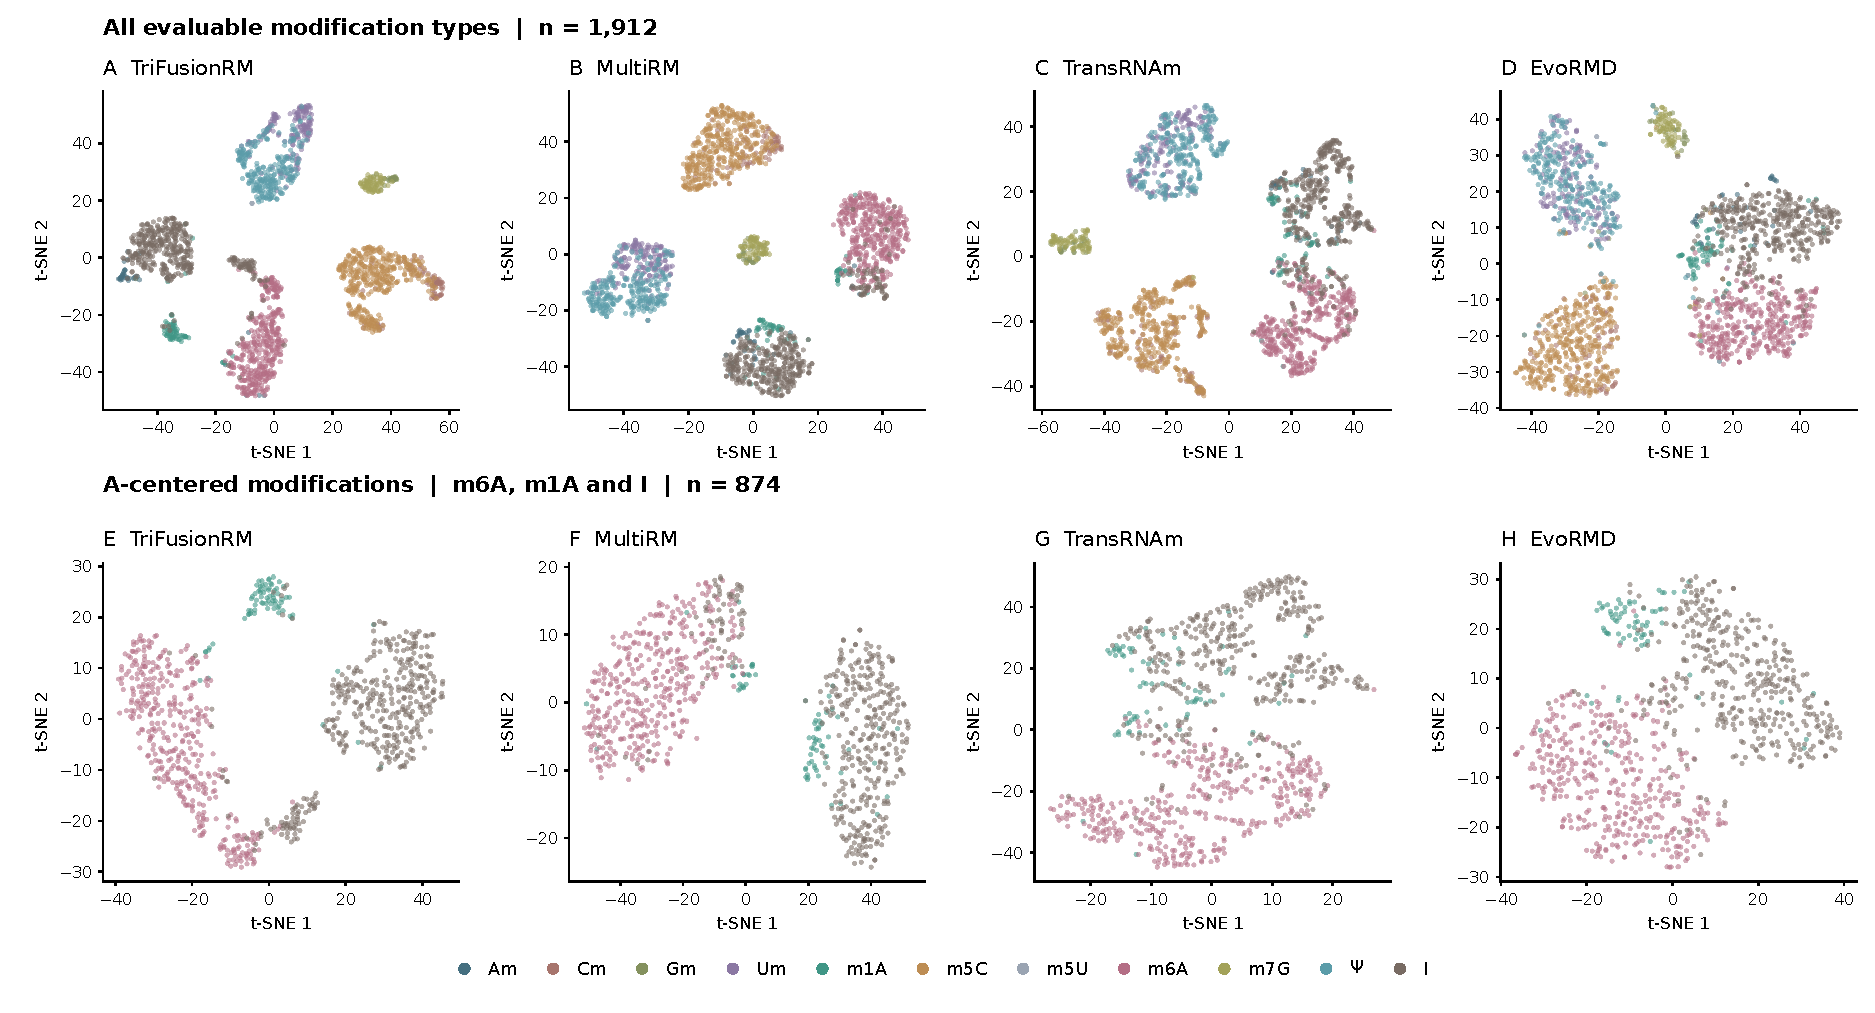
\includegraphics[width=\textwidth]{../figures/Figure6_logits_four_models.pdf}
\caption{t-SNE visualization of final classification scores from TriFusionRM and three benchmark implementations. Panels A--D show the same 1,912 internal test sites across eleven evaluable modification types. Panels E--H show the 874 A-centered m6A, m1A and I sites. Columns correspond to TriFusionRM, MultiRM, TransRNAm and EvoRMD. Each model contributes twelve final class logits per site, not a common intermediate embedding. Colors indicate annotated modification types. One site was selected per class and CD-HIT80 cluster, up to 400 sites per class, using sampling seed 42. Each panel was fitted independently with t-SNE perplexity 30, PCA initialization and random seed 42; axes and inter-panel distances are not directly comparable.}
\label{fig:tsne}
\end{figure*}

\section{Discussion}

We asked whether information beyond sequence improves classification among annotated RNA modification types. TriFusionRM combined three sequence lengths with predicted structure and positional RBP evidence. It outperformed the three evaluated benchmark implementations on the internal test set. The gain over sequence only also appeared in same-base analysis and in an external set containing six modification types. These findings support combining contextual inputs, although their benefit differs among classes.

Site-matched RBP profiles provided the clearest evidence beyond sequence. The full model outperformed the shuffled-RBP control, and adding RBP to sequence plus structure improved the overall score. These findings are consistent with previously reported associations among RNA modifications, RNA structure, and protein binding \citep{ref21}. eCLIP peaks also reflect transcript context and assay coverage, so these associations do not identify a causal RBP. We found no significant overall effect of changing the order of the six RBP distance intervals.

The independent contribution of predicted RNA structure was less consistent. Adding structure alone did not establish an overall gain after correction, and $\Psi$ AUPR decreased by 0.03395 relative to sequence only. One possible explanation is that binary pairing indicators from a 41-nt RNAfold window capture only local predicted folding, whereas the sequence encoder also uses 101- and 201-nt contexts. The shuffled-structure comparison does not resolve this mechanism, so the class-specific decrease should be treated as an observed model effect rather than evidence that RNA structure is biologically unimportant.

External performance also varied by modification. Relative to sequence only, TriFusionRM had lower AUPR for m6A (0.9790 to 0.9727), $\Psi$ (0.9999 to 0.9969) and m7G (0.9878 to 0.9735), whereas m5C remained 1.0000 at the reported precision (Table 4). The near-ceiling sequence-only scores for m6A, $\Psi$ and m5C left little room for improvement. For m7G, a change in the usefulness of structural or RBP context on the external sites is a possible explanation, but these results do not identify which input caused the decrease. The overall external gain therefore reflects larger improvements for I and m1A rather than a uniform benefit across classes.

The datasets have several limitations. We split the internal data using 41-nt clusters, so the longer 101-nt and 201-nt windows are not guaranteed to be independent across sets. A separate 101-nt screen found training matches for 41,257 of 107,618 distinct validation sequences at 80\% identity and coverage. The external filter also used 41-nt sequence similarity and cannot remove every possible shared context. The data are imbalanced, and some genomic coordinates have conflicting labels. m6Am has no positive internal test sites. The task distinguishes modification labels at annotated sites and does not use experimentally confirmed unmodified sites as a negative class. External gains were concentrated in I and m1A.

The identified motifs are associated with classes, and changing them affects predictions more than matched random changes. The perturbations changed sequence inputs while holding predicted structure and RBP features fixed. Experimental perturbations and measurements of RNA structure and RBP binding are needed to test biological mechanisms. Future benchmark work should also match training data and input information more closely across methods. 

\section{Conclusion}

TriFusionRM combines sequence context at three lengths with predicted RNA structure and positional RBP evidence to classify annotated RNA modification types. It achieved a Macro AUPR of 0.9297 across the 11 classes evaluable in the internal test set and 0.8085 across six classes in the external dataset. The combined model outperformed sequence-only prediction, although the benefit differed among modification types. Control experiments provided the clearest support for RBP features matched to individual sites, while predicted structure did not show a consistent independent benefit. 

\begin{thebibliography}{99}
\bibitem{ref1}Sun H, Li K, Liu C, et al. Regulation and functions of non-m6A mRNA modifications. Nature Reviews Molecular Cell Biology. 2023, 24, 714-731.
\bibitem{ref2}Meyer KD, Saletore Y, Zumbo P, et al. Comprehensive Analysis of mRNA Methylation Reveals Enrichment in 3' UTRs and near Stop Codons. Cell. 2012, 149, 1635-1646.
\bibitem{ref3}Linder B, Grozhik AV, Olarerin-George AO, et al. Single-nucleotide-resolution mapping of m6A and m6Am throughout the transcriptome. Nature Methods. 2015, 12, 767-772.
\bibitem{ref4}Zhang Y, Lu L, Li X. Detection technologies for RNA modifications. Experimental \& Molecular Medicine. 2022, 54, 1601-1616.
\bibitem{ref5}Hendra C, Pratanwanich PN, Wan YK, et al. Detection of m6A from direct RNA sequencing using a multiple instance learning framework. Nature Methods. 2022, 19, 1590-1598.
\bibitem{ref6}Acera Mateos P, J Sethi A, Ravindran A, et al. Prediction of m6A and m5C at single-molecule resolution reveals a transcriptome-wide co-occurrence of RNA modifications. Nature Communications. 2024, 15, 3899.
\bibitem{ref7}Wu Y, Shao W, Yan M, et al. Transfer learning enables identification of multiple types of RNA modifications using nanopore direct RNA sequencing. Nature Communications. 2024, 15, 4049.
\bibitem{ref8}Zhou Y, Zeng P, Li YH, et al. SRAMP: prediction of mammalian N6-methyladenosine (m6A) sites based on sequence-derived features. Nucleic Acids Research. 2016;44(10):e91.
\bibitem{ref9}Chen W, Tang H, Ye J, et al. iRNA-PseU -- Identifying RNA pseudouridine sites. Molecular Therapy - Nucleic Acids. 2016, 5, e332.
\bibitem{ref10}Chen K, Wei Z, Zhang Q, et al. WHISTLE: a high-accuracy map of the human N6-methyladenosine (m6A) epitranscriptome predicted using a machine learning approach. Nucleic Acids Research. 2019;47(7):e41.
\bibitem{ref11}Chen Z, Zhao P, Li F, et al. Comprehensive review and assessment of computational methods for predicting RNA post-transcriptional modification sites from RNA sequences. Briefings in Bioinformatics. 2020, 21, 1676-1696.
\bibitem{ref12}Zhuang J, Liu D, Lin M, et al. PseUdeep -- RNA Pseudouridine Site Identification with Deep Learning Algorithm. Frontiers in Genetics. 2021, 12, 773882.
\bibitem{ref13}Fan R, Cui C, Kang B, et al. A combined deep learning framework for mammalian m6A site prediction. Cell Genomics. 2024, 4, 100697.
\bibitem{ref14}Suto T, Harun-Or-Roshid M, Kurata H. Meta-PseU -- A meta-classifier for robust prediction of RNA pseudouridine modification sites from long sequences. Computer Methods and Programs in Biomedicine. 2026, 286, 109581.
\bibitem{ref15}Liu K, Chen W. iMRM -- a platform for simultaneously identifying multiple kinds of RNA modifications. Bioinformatics. 2020, 36, 3336-3342.
\bibitem{ref16}Song Z, Huang D, Song B, et al. Attention-based multi-label neural networks for integrated prediction and interpretation of twelve widely occurring RNA modifications. Nature Communications. 2021, 12, 4011.
\bibitem{ref17}Chen T, Wu T, Pan D, et al. TransRNAm -- Identifying Twelve Types of RNA Modifications by an Interpretable Multi-Label Deep Learning Model Based on Transformer. IEEE/ACM Transactions on Computational Biology and Bioinformatics. 2023, 20, 3623-3634.
\bibitem{ref18}Wang L, Zhou Y. MRM-BERT -- a novel deep neural network predictor of multiple RNA modifications by fusing BERT representation and sequence features. RNA Biology. 2024, 21, 340-349.
\bibitem{ref19}Wang B, Zhang H, Cui T, et al. EvoRMD -- integrating biological context and evolutionary RNA language models for interpretable prediction of RNA modifications. Genome Biology. 2026, 27, 204.
\bibitem{ref20}Cao X, Zhang Y, Ding Y, et al. Identification of RNA structures and their roles in RNA functions. Nature Reviews Molecular Cell Biology. 2024, 25, 784-801.
\bibitem{ref21}Lewis CJT, Pan T, Kalsotra A. RNA modifications and structures cooperate to guide RNA--protein interactions. Nature Reviews Molecular Cell Biology. 2017;18(3):202--210.
\bibitem{ref22}Lorenz R, Bernhart SH, Höner zu Siederdissen C, et al. ViennaRNA Package 2.0. Algorithms for Molecular Biology. 2011, 6, 26.
\bibitem{ref23}Van Nostrand EL, Pratt GA, Shishkin AA, et al. Robust transcriptome-wide discovery of RNA-binding protein binding sites with enhanced CLIP (eCLIP). Nature Methods. 2016, 13, 508-514.
\bibitem{ref24}Xuan J, Chen L, Chen Z, et al. RMBase v3.0 -- decode the landscape, mechanisms and functions of RNA modifications. Nucleic Acids Research. 2024, 52, D273-D284.
\bibitem{ref25}Li W, Godzik A. Cd-hit -- a fast program for clustering and comparing large sets of protein or nucleotide sequences. Bioinformatics. 2006, 22, 1658-1659.
\bibitem{ref26}Frankish A, Diekhans M, Ferreira AM, et al. GENCODE reference annotation for the human and mouse genomes. Nucleic Acids Research. 2019, 47, D766-D773.
\bibitem{ref27}Luo T, Xu M, Wang M, et al. Systematic evaluation of computational tools for multitype RNA modification detection using nanopore direct RNA sequencing. Nature Methods. 2026, 23, 438-450.
\bibitem{ref28}Steinegger M, Söding J. Clustering huge protein sequence sets in linear time. Nature Communications. 2018, 9, 2542.
\bibitem{ref29}Hendrycks D, Gimpel K. Gaussian Error Linear Units (GELUs). arXiv. 2016, 1606.08415.
\bibitem{ref30}Ba JL, Kiros JR, Hinton GE. Layer Normalization. arXiv. 2016, 1607.06450.
\bibitem{ref31}Cho K, van Merrienboer B, Gulcehre C, et al. Learning Phrase Representations using RNN Encoder--Decoder for Statistical Machine Translation. Proceedings of the 2014 Conference on Empirical Methods in Natural Language Processing (EMNLP). 2014, 1724-1734.
\bibitem{ref32}Veličković P, Cucurull G, Casanova A, et al. Graph Attention Networks. International Conference on Learning Representations. 2018.
\bibitem{ref33}Loshchilov I, Hutter F. Decoupled Weight Decay Regularization. International Conference on Learning Representations. 2019.
\bibitem{ref34}Pedregosa F, Varoquaux G, Gramfort A, et al. Scikit-learn -- Machine Learning in Python. Journal of Machine Learning Research. 2011, 12, 2825-2830.
\bibitem{ref35}Matthews BW. Comparison of the predicted and observed secondary structure of T4 phage lysozyme. Biochimica et Biophysica Acta (BBA) - Protein Structure. 1975;405(2):442--451.
\bibitem{ref36}Harden JJ. A Bootstrap Method for Conducting Statistical Inference with Clustered Data. State Politics \& Policy Quarterly. 2011, 11, 223-246.
\bibitem{ref37}Benjamini Y, Hochberg Y. Controlling the False Discovery Rate -- A Practical and Powerful Approach to Multiple Testing. Journal of the Royal Statistical Society: Series B. 1995, 57, 289-300.
\bibitem{ref38}Cui Y, Jia M, Lin TY, et al. Class-Balanced Loss Based on Effective Number of Samples. Proceedings of the IEEE/CVF Conference on Computer Vision and Pattern Recognition (CVPR). 2019:9268--9277.
\end{thebibliography}
\end{document}
